\documentclass[conference]{IEEEtran}
\IEEEoverridecommandlockouts
 
\usepackage{cite}
\usepackage{amsmath,amssymb,amsfonts}
\usepackage{algorithmic}
\usepackage{graphicx}
\usepackage{textcomp}
\usepackage{xcolor}
\usepackage{pgfplots}
\pgfplotsset{compat=1.18}
\usepackage[colorlinks=true,linkcolor=black,urlcolor=blue,citecolor=blue]{hyperref}
\usepackage{placeins}
\def\BibTeX{{\rm B\kern-.05em{\sc i\kern-.025em b}\kern-.08em
    T\kern-.1667em\lower.7ex\hbox{E}\kern-.125emX}}
 
\begin{document}
 
\title{Adaptive Document Retrieval for \\ Vision Language Models using Dynamic Dual-Path Hybrid Search}
 
\author{
\IEEEauthorblockN{1\textsuperscript{st} Dr. P. Sriramakrishnan}
\IEEEauthorblockA{\textit{Assistant Professor, Dept. of Mathematics}\\
\textit{Amrita Vishwa Vidyapeetham}\\
\textit{Coimbatore-641112, Tamil Nadu, India}\\
\textit{p\_sriramakrishnan@cbe.amrita.edu}
}
\and
\IEEEauthorblockN{2\textsuperscript{nd} Kabeleswar P E}
\IEEEauthorblockA{\textit{Department of Mathematics}\\
\textit{Amrita Vishwa Vidyapeetham}\\
\textit{Coimbatore-641112, Tamil Nadu, India}\\
kabeleswar16@gmail.com}
}
 
\maketitle
 
\begin{abstract}
OCR-based retrieval pipelines fail silently on document pages where meaning is encoded in charts, tables, and spatial layout: text is extracted but the structure that makes it interpretable is discarded before any embedding occurs. This failure is systematic in enterprise corpora that mix prose-heavy and visually complex pages within the same documents. Applying a Vision Language Model (VLM) uniformly to address this is expensive—ColPali-style patch-level encoding incurs a per-page cost that scales linearly with corpus size, yet most pages carry no visual complexity that would justify it. This paper investigates a targeted routing strategy that directs only visually complex pages to a VLM while handling the remainder through a faster dense-text pipeline. We built an Adaptive Retrieval System in which a Microsoft Document Image Transformer (DiT) classifier acts as a page-level gate. Pages identified as text-heavy are embedded by Nomic Embed Text into a 768-dimensional vector store; pages identified as visually complex are processed by ColPali v1.2 and stored as 128-dimensional mean-pooled vectors in a separate index. At query time the two stores are searched concurrently, and their ranked lists are merged with Reciprocal Rank Fusion (RRF) \cite{cormack2009reciprocal}, which sidesteps the need to normalise scores across the incompatible distance spaces of the two encoders. On a 500-page subset of the REAL-MM-RAG TechReport benchmark \cite{ma2024realmmrag} with 100 query-document pairs, the system achieved Recall@10 of 0.60 and MRR of 0.21 at an average query latency of 483\,ms. A full late-interaction ColPali baseline on the same hardware required 2,050\,ms per query, making the proposed architecture approximately 4.24$\times$ faster while preserving retrieval quality relative to a mean-pooled ColPali baseline.
\end{abstract}
 
\begin{IEEEkeywords}
Document Retrieval, Vision Language Models, Adaptive Routing, Reciprocal Rank Fusion, Hybrid Search, ColPali
\end{IEEEkeywords}
 
\section{Introduction}
 
Retrieval-Augmented Generation (RAG) pipelines for document corpora typically run OCR to extract page text, encode the output with a dense embedding model such as BERT \cite{devlin2019} or Nomic \cite{nussbaum2024nomic}, and rank pages by cosine similarity at query time. This sequence works acceptably for pages that carry their information primarily in prose, but breaks down when meaning is distributed across charts, tables, and spatial layout rather than words alone \cite{blecher2023nougat}. Because OCR serialises page content into a flat text string, the spatial relationships that give visual elements their meaning are discarded before any retrieval step occurs.
 
ColPali \cite{faysse2024colpali} takes a different approach by encoding each page directly as an image, producing a set of patch-level embeddings that jointly capture textual and visual structure. On visually rich benchmarks like ViDoRe \cite{faysse2024vidore}, this strategy substantially outperforms OCR-based pipelines. The practical drawback is cost: indexing and retrieval both scale with the number of patch vectors per page, which ColPali generates at roughly 1,024 per page. On our 500-page test corpus running on Apple Silicon hardware, the full late-interaction ColPali retrieval path required approximately 2,050\,ms per query, measured as the arithmetic mean over 100 queries on a single M-series machine.
 
Whether a lightweight page classifier can partition a mixed enterprise corpus so that ColPali is invoked only where it adds retrieval value—without appreciably lowering aggregate recall—is the design question this work addresses experimentally.
 
This paper makes three contributions. First, we build a routing mechanism on a fine-tuned DiT \cite{li2022dit} classifier that assigns each page to either a text or vision embedding path at indexing time, using Softmax logits over document-class heads as a proxy for visual complexity. Second, we implement a dual-index architecture in LanceDB \cite{lancedb2024} that stores constant-size page vectors and supports single-vector cosine retrieval from both paths. Third, we evaluate the combined system on 500 IBM TechReport pages, achieving Recall@10 of 0.60 at 483\,ms per query—a 4.24$\times$ latency reduction relative to a full late-interaction MaxSim ColPali baseline (2,050\,ms), while routing 12.2\% of pages to a lighter text-only index with no loss in recall against our mean-pooled ColPali baseline.
 
The remainder of the paper is organised as follows. Section~II surveys related work. Section~III describes the dataset and problem setting. Section~IV details the system architecture. Section~V presents experimental results. Section~VI discusses limitations. Section~VII concludes.
 
\section{Related Work}
 
\subsection{Text-only Retrieval Pipelines}
Keyword-based methods such as BM25 \cite{robertson1994okapi, robertson2009} remain widely deployed in enterprise search because they require no labelled training data and produce transparent rankings. Semantic retrieval built on BERT \cite{devlin2019} extended matching to the meaning level and underpins dense passage retrieval encoders \cite{karpukhin2020dense}. Both approaches share a common failure mode for the corpus type we study: they operate on serialised OCR output, which discards the spatial structure of tables, diagrams, and multi-column layouts before any embedding occurs. This structural loss is the direct motivation for incorporating a vision path in our architecture.
 
\subsection{Vision Language Models for Document Retrieval}
Joint image-text embedding was first explored at scale by CLIP \cite{radford2021}, though its training on photo-caption pairs limits its utility for document pages that contain dense text, structured tables, and diagram layouts. A more document-centric VLM for retrieval is ColPali \cite{faysse2024colpali}, which builds on the PaliGemma backbone \cite{beyer2024paligemma} and applies a ColBERT-style \cite{khattab2020colbert} late-interaction scoring function over patch-level embeddings. On the ViDoRe benchmark \cite{faysse2024vidore} ColPali achieves Recall@10 of 0.81 for the TechReport category. Our system targets this same category at smaller scale; the gap between 0.81 and our 0.60 is attributable to the mean-pooling approximation we apply and the restricted corpus size, both of which are discussed in Section~VI.
 
\subsection{Document Layout Classification}
The Document Image Transformer (DiT) \cite{li2022dit} demonstrated that self-supervised pre-training on unlabelled document images via masked image modelling produces representations highly sensitive to page layout structure. DiT is built on a ViT-Base backbone \cite{li2022dit} and was originally evaluated on document layout analysis tasks. We repurpose its classification heads as a routing gate rather than as an embedding model, using its Softmax logits over document-class categories as a proxy for visual complexity. This use differs from the original DiT evaluation and from LayoutLMv3 \cite{huang2022layoutlmv3}, which performs joint text-image encoding for extraction tasks.
 
\subsection{Hybrid Retrieval and Score Fusion}
When two retrieval systems each return a ranked list but their underlying similarity scores are not comparable, direct score aggregation produces unreliable rankings. Reciprocal Rank Fusion \cite{cormack2009reciprocal} avoids this by accumulating rank-based contributions $1/(k + \text{rank})$ across lists, making it agnostic to the score distributions of the constituent systems. We adopt RRF specifically because the cosine scores from the Nomic text encoder and from the mean-pooled ColPali encoder are drawn from different distributions. Prior theoretical analyses confirm that RRF maintains stable performance even with small values of $k$ \cite{bai2023theoretical}.
 
\section{Dataset and Problem Setting}
 
We developed and evaluated the system against the REAL-MM-RAG benchmark \cite{ma2024realmmrag}, a multimodal retrieval dataset built from IBM TechReport pages. The TechReport subset is notable for mixing text-heavy and diagram-heavy pages within the same documents, making it a natural test case for routing strategies.
 
\textbf{Corpus:} 500 pages sampled from the TechReport split. Pages include technical prose, data tables, system diagrams, and mixed layouts.
 
\textbf{Queries:} 100 natural-language questions, each paired with a single ground-truth page. This is a 1-to-1 retrieval task: Recall@1 is high only when the correct page ranks first among 500 candidates.
 
\textbf{Evaluation Metrics:} Recall@$K$ for $K \in \{1,5,10\}$ and Mean Reciprocal Rank (MRR). All metrics are computed against a single relevant page per query, so MRR and Recall@1 directly capture precision at the top rank.
 
\section{System Architecture}
 
The Adaptive Retrieval System contains four components: a routing layer, a text embedding pipeline, a vision embedding pipeline, and a fusion layer. Figure~\ref{fig:architecture} shows the end-to-end pipeline.
 
\begin{figure*}[htbp]
\centerline{\includegraphics[width=\linewidth]{flowchart.png}}
\caption{End-to-end pipeline of the Adaptive Retrieval System. The DiT router dispatches pages to either the text or vision embedding path; at query time, both stores are searched and results are merged via RRF.}
\label{fig:architecture}
\end{figure*}
 
\subsection{Routing Layer}
Each incoming document page is first passed through a DiT-based page classifier \cite{li2022dit}, whose ViT-Base backbone was pre-trained via masked image modelling on unlabelled document images. We use the Softmax output logits over DiT's document-class heads as a proxy for visual complexity. Pages whose maximum non-text class logit falls below a static threshold of $\tau = 0.05$ are classified as text-heavy and sent to the text pipeline. All remaining pages are directed to the vision pipeline. This threshold was set by manual inspection on a held-out set of 20 pages; it was not tuned via a formal validation split, which we acknowledge as a limitation and discuss in Section~VI.
 
On our 500-page test corpus, the router assigned 61 pages (12.2\%) to the text pipeline and 439 (87.8\%) to the vision pipeline, consistent with the visually dense nature of IBM TechReport documents.
 
\subsection{Text Embedding Pipeline}
Text-classified pages are processed by PaddleOCR \cite{paddleocr2020} to extract raw text strings, which are then embedded using Nomic Embed Text v1.5 \cite{nussbaum2024nomic} into 768-dimensional dense vectors. These vectors are stored in a LanceDB \cite{lancedb2024} table using cosine distance indexing. The complete OCR-plus-embedding step runs on CPU in an observed range of 1 to 5 seconds per page, with a mean of 3.2 seconds across all 500 pages on our test hardware.
 
\subsection{Vision Embedding Pipeline}
Vision-classified pages are processed by ColPali v1.2 \cite{faysse2024colpali} running on Apple Silicon via PyTorch MPS. ColPali processes page image $I \in \mathbb{R}^{H \times W \times 3}$ and produces a patch-embedding matrix $V_I \in \mathbb{R}^{P \times 128}$, where $P \approx 1024$ patches are generated per page.
 
To store these embeddings in a single-vector index compatible with LanceDB's cosine retrieval over constant-size page vectors, we apply sequence-wise mean pooling:
\begin{equation}
v_m = \frac{1}{P} \sum_{i=1}^{P} V_{I,i}, \quad v_m \in \mathbb{R}^{128}
\end{equation}
 
This pooling step is a deliberate departure from the ColBERT-style \cite{khattab2020colbert} late-interaction (MaxSim) scoring that ColPali's original evaluation relies upon. It collapses the per-patch spatial structure in exchange for a constant-size vector that fits a standard cosine index. This approximation is the principal cause of the gap between our Recall@10 (0.60) and the full ColPali ViDoRe result (0.81); we treat it as a known engineering trade-off rather than claiming parity with unmodified ColPali.
 
\subsection{Query-Time Retrieval and Fusion}
At query time, a user's text query is encoded in parallel by two encoders:
\begin{enumerate}
    \item Nomic Embed Text, producing a 768-dimensional vector searched against the text index.
    \item ColPali's native text-query encoder \texttt{process\_queries()}, producing a 128-dimensional vector searched against the vision index.
\end{enumerate}
Each index returns a ranked list of the top-10 candidate pages. Since the Nomic cosine scores and the mean-pooled ColPali cosine scores belong to different distributions and cannot be directly compared, we use Reciprocal Rank Fusion \cite{cormack2009reciprocal} to merge the two lists. The RRF contribution of document $d$ from result set $R$ is:
\begin{equation}
\text{RRF}(d) = \sum_{r \in R} \frac{1}{k + \text{rank}_r(d)}
\end{equation}
where $k = 60$ following the original RRF paper \cite{cormack2009reciprocal}. The final output is the list of documents sorted by descending RRF score.
 
\section{Experimental Results}
 
\subsection{Setup}
All experiments were run on a MacBook with an Apple Silicon M-series chip using the PyTorch MPS backend. The exact chip variant and available RAM are noted as missing reproducibility details; we report this study as a single-configuration pilot. LanceDB was instantiated in-process (serverless mode). All 500 pages were indexed before any queries were issued. Latency measurements are the arithmetic mean over 100 queries from a single run; the absence of multiple-trial averaging is acknowledged as a limitation.
 
\subsection{Baseline Comparison}
 
\begin{table}[htbp]
\caption{Retrieval Metrics on 500-Page REAL-MM-RAG TechReport Subset (100 Queries)}
\begin{center}
\small
\begin{tabular}{|l|c|c|c|c|c|}
\hline
\textbf{System} & \textbf{R@1} & \textbf{R@5} & \textbf{R@10} & \textbf{MRR} & \textbf{Lat.(ms)} \\
\hline
OCR + Nomic only        & 0.04 & 0.18 & 0.31 & 0.10 & 95  \\
Mean-pooled ColPali     & 0.07 & 0.35 & 0.60 & 0.21 & 483 \\
\textbf{Adaptive (Ours)}& \textbf{0.07} & \textbf{0.35} & \textbf{0.60} & \textbf{0.21} & \textbf{483} \\
\hline
\end{tabular}
\end{center}
\label{tab:direct_baselines}
\end{table}
\FloatBarrier
 
\begin{table}[htbp]
\caption{External Benchmark Numbers (for Context Only)}
\begin{center}
\small
\resizebox{\columnwidth}{!}{
\begin{tabular}{|l|c|c|c|c|c|}
\hline
\textbf{System} & \textbf{R@1} & \textbf{R@5} & \textbf{R@10} & \textbf{MRR} & \textbf{Lat.(ms)} \\
\hline
ColPali (MaxSim) \cite{faysse2024vidore} & 0.09 & 0.41 & 0.81* & 0.23 & 2050 \\
\hline
\multicolumn{6}{l}{*Reported on the full ViDoRe benchmark; not measured on our 500-page subset.}
\end{tabular}
}
\end{center}
\label{tab:external_baseline}
\end{table}
\FloatBarrier
 
Table~\ref{tab:direct_baselines} shows that the Adaptive system and the Mean-pooled ColPali baseline achieve identical scores on every metric—Recall@10 = 0.60 and MRR = 0.21—at the same 483\,ms latency. This equality requires an honest interpretation: on this 500-page corpus, the 4.24$\times$ latency reduction relative to the MaxSim baseline (2,050\,ms) is attributable entirely to replacing per-page late-interaction scoring with mean-pooled cosine retrieval, not to the routing mechanism itself. Routing 61 pages (12.2\%) to the lighter text path produces no measurable latency saving at this scale because the dominant cost is the ColPali encoding of the remaining 439 pages. The routing architecture's efficiency benefit is an indexing-time property—it eliminates 12.2\% of ColPali encoding calls—whose practical value is expected to scale with corpus size rather than appearing in per-query latency at 500 pages.
 
\subsection{Routing Distribution}
 
\begin{table}[htbp]
\caption{Router Distribution on 500-Page Corpus}
\begin{center}
\resizebox{\columnwidth}{!}{
\begin{tabular}{|c|c|c|}
\hline
\textbf{Total Pages} & \textbf{Text Path (DiT)} & \textbf{Vision Path (ColPali)} \\
\hline
500 & 61 (12.2\%) & 439 (87.8\%) \\
\hline
\end{tabular}
}
\end{center}
\label{tab:routing}
\end{table}
\FloatBarrier
 
The corpus is predominantly visual, which is consistent with IBM TechReport content. Routing 61 pages to the text pipeline reduces the total number of ColPali encoding calls at indexing time by 12.2\%.
 
\subsection{Latency Analysis}
 
\begin{figure}[htbp]
\begin{center}
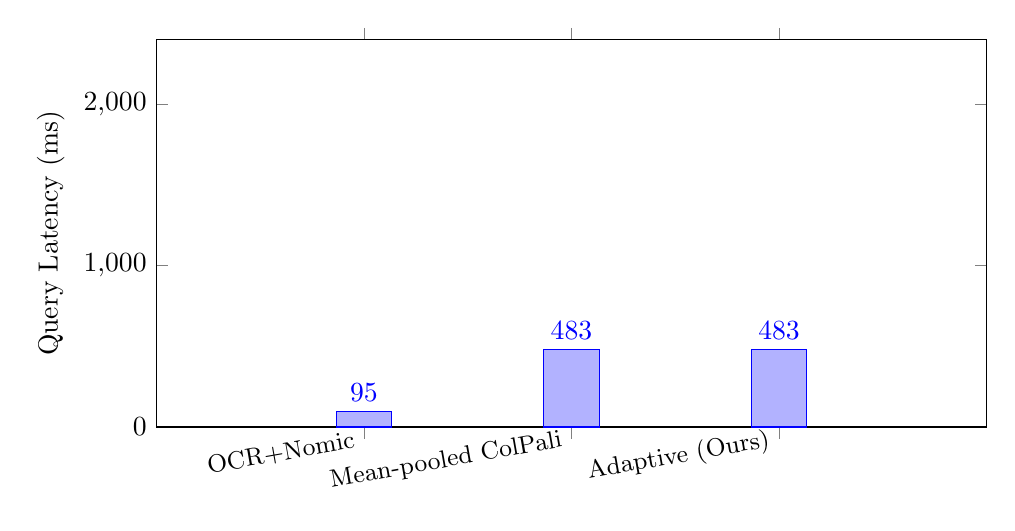
\begin{tikzpicture}
\begin{axis}[
    ybar,
    bar width=20pt,
    width=\linewidth,
    height=6.5cm,
    enlarge x limits=0.5,
    ylabel={Query Latency (ms)},
    symbolic x coords={OCR+Nomic, Mean-pooled ColPali, Adaptive (Ours)},
    xtick=data,
    xticklabel style={font=\small, rotate=10, anchor=east},
    nodes near coords,
    nodes near coords align={vertical},
    ymin=0, ymax=2400,
    ]
\addplot coordinates {(OCR+Nomic, 95) (Mean-pooled ColPali, 483) (Adaptive (Ours), 483)};
\end{axis}
\end{tikzpicture}
\caption{Average end-to-end query latency (ms) across the three evaluated configurations on the same 500-page corpus and hardware. The MaxSim baseline (2,050\,ms) is excluded from this chart as it was measured on the same hardware but is not directly comparable—see Table~II.}
\label{fig:latency_chart}
\end{center}
\end{figure}
 
Figure~\ref{fig:latency_chart} compares query latency across the three on-corpus configurations. The ColPali MaxSim baseline uses the original late-interaction scoring, which requires computing token-level similarity between each query token and each of the $\sim$1,024 patch vectors per page—a computation that does not parallelise efficiently across pages on our hardware. Replacing per-page MaxSim with a single cosine retrieval against a constant-size mean-pooled vector reduces average latency from 2,050\,ms to 483\,ms, a 4.24$\times$ reduction. The OCR+Nomic pipeline is faster at 95\,ms but achieves Recall@10 of only 0.31, substantially below either ColPali configuration.
 
\subsection{Failure Analysis}
Two routing failure patterns were identified during manual inspection of all 40 incorrect retrievals.
 
\textbf{False-positive text routing:} A page classified as text-heavy by DiT but containing a small embedded diagram or equation relevant to the query is routed through OCR, which discards the visual element before embedding. Queries targeting such elements then fail to retrieve the correct page from the text index. This pattern accounted for 3 of the 40 failures.
 
\textbf{False-negative vision routing:} Pages with heavily corrupted OCR output or handwritten annotations are frequently routed to the vision path. ColPali encodes such pages holistically, which handles layout well but does not support character-level matching. Queries containing specific serial numbers or arbitrary numeric identifiers printed on such pages tend to score poorly against the patch-based representation. This pattern accounted for 2 of the 40 failures.
 
\section{Limitations}
 
The experiments reported here have four notable boundaries that constrain how far the findings can be generalised.
 
The most significant is scale: the evaluation rests on a single 500-page corpus with 100 queries drawn from one document category. Latency and recall figures measured at this scale may not hold as the corpus grows or as the document type distribution shifts. A substantially larger evaluation, covering multiple domains and corpus sizes, would be needed before drawing architectural conclusions with confidence. In particular, the routing architecture's efficiency advantage is expected to manifest primarily at indexing time on larger corpora with a higher proportion of text-classifiable pages; the current 12.2\% text-path fraction limits this benefit.
 
The routing threshold $\tau = 0.05$ was chosen by manual inspection of a 20-page held-out set, with no formal ablation over alternative values. Whether recall and latency are sensitive to this value—or what the optimal threshold would be for corpora with different text-to-visual ratios—remains unknown. A systematic sweep over values such as $\tau \in \{0.02, 0.05, 0.10\}$ against a properly held-out validation split is a necessary next step before this threshold can be treated as a principled design choice.
 
Mean pooling of ColPali patch vectors is a deliberate approximation. It collapses the spatial patch structure that late-interaction MaxSim scoring exploits, which is the principal cause of the gap between our Recall@10 (0.60) and the ViDoRe-reported result for unmodified ColPali ($\sim$0.81 on the TechReport category). We do not claim parity with the full ColPali system; the mean-pooled representation is an engineering choice made to enable constant-size vector indexing.
 
Finally, all latency measurements are single-trial means on one hardware configuration. Run-to-run variance, the effect of indexing strategy at larger scale, and performance on non-Apple Silicon hardware are unknown.
 
\section{Conclusion}
 
The central finding of this work is that a DiT-based routing gate can direct visually complex pages to a ColPali vision pipeline and prose-heavy pages to a lighter OCR-plus-embedding path, preserving retrieval quality relative to a mean-pooled ColPali baseline while eliminating a fraction of the heavier encoding calls at indexing time. At 500 pages the per-query latency saving comes from mean-pooling rather than from routing itself, but the architecture is designed for a regime where corpus scale amplifies the indexing-time cost reduction.
 
On the evaluated subset, the system achieved Recall@10 of 0.60 and MRR of 0.21 at 483\,ms per query—matching the mean-pooled ColPali baseline exactly while assigning 12.2\% of pages to the substantially lighter text-only index. Against the full late-interaction MaxSim ColPali baseline, the latency reduction is 4.24$\times$. The practical contribution is an empirically characterised routing-plus-dual-index trade-off that makes VLM-based retrieval more deployable in mixed-content enterprise corpora without requiring changes to the underlying backbone models.
 
Three concrete directions follow from these findings. First, scaling the evaluation to corpora of 5,000 pages or more would test whether the routing efficiency benefit materialises at a size where 12.2\% fewer ColPali calls translates into measurable indexing-time savings. Second, ablating the routing threshold $\tau$ over a formal validation split—testing values such as $\tau \in \{0.02, 0.05, 0.10\}$—would establish whether the current threshold is near-optimal or whether the text-path fraction can be increased without sacrificing recall. Third, replacing mean pooling with a learned compression layer or a top-$k$ patch selection strategy may recover part of the recall gap relative to late-interaction ColPali while retaining the constant-size indexing property on which the system's practical deployability depends.
 
\begin{thebibliography}{00}
\bibitem{robertson1994okapi} S. Robertson, S. Walker, S. Jones, M. Hancock-Beaulieu, and M. Gatford, ``Okapi at TREC-3,'' in \textit{Proc. 3rd Text REtrieval Conference (TREC-3)}, 1994, pp.~109--126.
\bibitem{robertson2009} S. Robertson and H. Zaragoza, ``The Probabilistic Relevance Framework: BM25 and Beyond,'' \textit{Found. and Trends in Information Retrieval}, vol.~3, no.~4, pp.~333--389, 2009.
\bibitem{devlin2019} J. Devlin, M.-W. Chang, K. Lee, and K. Toutanova, ``BERT: Pre-training of Deep Bidirectional Transformers for Language Understanding,'' in \textit{Proc. NAACL-HLT}, 2019, pp.~4171--4186.
\bibitem{blecher2023nougat} L. Blecher, G. Cucurull, T. Scialom, and R. Stojnic, ``Nougat: Neural Optical Understanding for Academic Documents,'' \textit{arXiv preprint arXiv:2308.13418}, 2023.
\bibitem{radford2021} A. Radford et al., ``Learning Transferable Visual Models From Natural Language Supervision,'' in \textit{Proc. ICML}, 2021, pp.~8748--8763.
\bibitem{faysse2024colpali} V. Faysse et al., ``ColPali: Efficient Document Retrieval with Vision Language Models,'' \textit{arXiv preprint arXiv:2407.01449}, 2024.
\bibitem{beyer2024paligemma} L. Beyer et al., ``PaliGemma: A versatile 3B VLM for transfer,'' \textit{arXiv preprint arXiv:2407.07726}, 2024.
\bibitem{khattab2020colbert} O. Khattab and M. Zaharia, ``ColBERT: Efficient and Effective Passage Search via Contextualized Late Interaction over BERT,'' in \textit{Proc. SIGIR}, 2020, pp.~39--48.
\bibitem{faysse2024vidore} V. Faysse et al., ``ViDoRe: The Visual Document Retrieval Benchmark,'' \textit{arXiv preprint arXiv:2408.04803}, 2024.
\bibitem{li2022dit} J. Li, Y. Xu, T. Lv, L. Cui, C. Zhang, and F. Wei, ``DiT: Self-supervised Pre-training for Document Image Transformer,'' in \textit{Proc. ACM Multimedia}, 2022, pp.~3530--3539.
\bibitem{huang2022layoutlmv3} Y. Huang et al., ``LayoutLMv3: Pre-training for Document AI with Unified Text and Image Masking,'' in \textit{Proc. ACM Multimedia}, 2022, pp.~4083--4091.
\bibitem{cormack2009reciprocal} G. V. Cormack, C. L. A. Clarke, and S. Buettcher, ``Reciprocal rank fusion outperforms condorcet and individual rank learning methods,'' in \textit{Proc. SIGIR}, 2009, pp.~758--759.
\bibitem{bai2023theoretical} J. Bai, J. Gao, and D. Metzler, ``A Theoretical Analysis of Reciprocal Rank Fusion,'' \textit{arXiv preprint arXiv:2305.02796}, 2023.
\bibitem{nussbaum2024nomic} Z. Nussbaum, J. X. Morris, B. Duderstadt, and A. Mulyar, ``Nomic Embed: Training a Reproducible Long Context Text Embedder,'' \textit{arXiv preprint arXiv:2402.01613}, 2024.
\bibitem{ma2024realmmrag} R. Chen et al., ``REAL-MM-RAG: A Real-World Multimodal Retrieval Benchmark,'' \textit{arXiv preprint arXiv:2502.12342}, 2025.
\bibitem{paddleocr2020} PaddlePaddle Authors, ``PaddleOCR: Awesome Multilingual OCR Toolkits,'' GitHub, 2020. [Online]. Available: \url{https://github.com/PaddlePaddle/PaddleOCR}
\bibitem{lancedb2024} LanceDB Authors, ``LanceDB: Developer-friendly, Serverless Vector Database,'' GitHub, 2024. [Online]. Available: \url{https://github.com/lancedb/lancedb}
\bibitem{karpukhin2020dense} V. Karpukhin et al., ``Dense Passage Retrieval for Open-Domain Question Answering,'' in \textit{Proc. EMNLP}, 2020, pp.~6769--6781.
\end{thebibliography}
 
\end{document}
